%%%%%%%%%%%%%%%%%%%%%%%%%%%%%%%%%%%%%%%%%
% Masters/Doctoral Thesis 
% LaTeX Template
% Version 2.5 (27/8/17)
%
% This template was downloaded from:
% http://www.LaTeXTemplates.com
%
% Version 2.x major modifications by:
% Vel (vel@latextemplates.com)
%
% This template is based on a template by:
% Steve Gunn (http://users.ecs.soton.ac.uk/srg/softwaretools/document/templates/)
% Sunil Patel (http://www.sunilpatel.co.uk/thesis-template/)
%
% Template license:
% CC BY-NC-SA 3.0 (http://creativecommons.org/licenses/by-nc-sa/3.0/)
%
%%%%%%%%%%%%%%%%%%%%%%%%%%%%%%%%%%%%%%%%%

%----------------------------------------------------------------------------------------
%	PACKAGES AND OTHER DOCUMENT CONFIGURATIONS
%----------------------------------------------------------------------------------------

\documentclass[
11pt, % The default document font size, options: 10pt, 11pt, 12pt
oneside, % Two side (alternating margins) for binding by default, uncomment to switch to one side
english, % ngerman for German
doublespacing, % Single line spacing, alternatives: onehalfspacing or doublespacing
%draft, % Uncomment to enable draft mode (no pictures, no links, overfull hboxes indicated)
%nolistspacing, % If the document is onehalfspacing or doublespacing, uncomment this to set spacing in lists to single
%liststotoc, % Uncomment to add the list of figures/tables/etc to the table of contents
%toctotoc, % Uncomment to add the main table of contents to the table of contents
%parskip, % Uncomment to add space between paragraphs
%nohyperref, % Uncomment to not load the hyperref package
headsepline, % Uncomment to get a line under the header
%chapterinoneline, % Uncomment to place the chapter title next to the number on one line
%consistentlayout, % Uncomment to change the layout of the declaration, abstract and acknowledgements pages to match the default layout
]{MastersDoctoralThesis} % The class file specifying the document structure

\usepackage[utf8]{inputenc} % Required for inputting international characters
\usepackage[T1]{fontenc} % Output font encoding for international characters

\usepackage{mathpazo} % Use the Palatino font by default

\usepackage[backend=bibtex,style=numeric,natbib=true]{biblatex} % Use the bibtex backend with the authoryear citation style (which resembles APA)

\addbibresource{Legacy.bib} % The filename of the bibliography

\usepackage[autostyle=true]{csquotes} % Required to generate language-dependent quotes in the bibliography

%----------------------------------------------------------------------------------------
%	MARGIN SETTINGS
%----------------------------------------------------------------------------------------

\geometry{
	paper=a4paper, % Change to letterpaper for US letter
	inner=2.5cm, % Inner margin
	outer=2.5cm, % Outer margin
	bindingoffset=.5cm, % Binding offset
	top=1.5cm, % Top margin
	bottom=1.5cm, % Bottom margin
	%showframe, % Uncomment to show how the type block is set on the page
}

%----------------------------------------------------------------------------------------
%	THESIS INFORMATION
%----------------------------------------------------------------------------------------

\thesistitle{Mutational Patterns in Founder Populations} % Your thesis title, this is used in the title and abstract, print it elsewhere with \ttitle
\supervisor{Dr. Simon \textsc{Gravel}} % Your supervisor's name, this is used in the title page, print it elsewhere with \supname
\examiner{} % Your examiner's name, this is not currently used anywhere in the template, print it elsewhere with \examname
\degree{Doctor of Philosophy} % Your degree name, this is used in the title page and abstract, print it elsewhere with \degreename
\author{Luke \textsc{Anderson-Trocm\'e}} % Your name, this is used in the title page and abstract, print it elsewhere with \authorname
\addresses{} % Your address, this is not currently used anywhere in the template, print it elsewhere with \addressname

\subject{Statistical Population Genetics} % Your subject area, this is not currently used anywhere in the template, print it elsewhere with \subjectname
\keywords{} % Keywords for your thesis, this is not currently used anywhere in the template, print it elsewhere with \keywordnames
\university{\href{http://www.mcgill.ca}{McGill University}} % Your university's name and URL, this is used in the title page and abstract, print it elsewhere with \univname
\department{\href{https://www.mcgill.ca/humangenetics/}{Department of Human Genetics}} % Your department's name and URL, this is used in the title page and abstract, print it elsewhere with \deptname
\group{\href{http://simongravel.lab.mcgill.ca/Home.html}{Gravel Lab}} % Your research group's name and URL, this is used in the title page, print it elsewhere with \groupname
\faculty{\href{https://www.mcgill.ca/medicine/}{Faculty of Medecine}} % Your faculty's name and URL, this is used in the title page and abstract, print it elsewhere with \facname

\AtBeginDocument{
\hypersetup{pdftitle=\ttitle} % Set the PDF's title to your title
\hypersetup{pdfauthor=\authorname} % Set the PDF's author to your name
\hypersetup{pdfkeywords=\keywordnames} % Set the PDF's keywords to your keywords
}

\begin{document}

\frontmatter % Use roman page numbering style (i, ii, iii, iv...) for the pre-content pages

\pagestyle{plain} % Default to the plain heading style until the thesis style is called for the body content

%----------------------------------------------------------------------------------------
%	TITLE PAGE
%----------------------------------------------------------------------------------------

\begin{titlepage}
\begin{center}

\vspace*{.06\textheight}
{\scshape\LARGE \univname\par}\vspace{1.5cm} % University name
\textsc{\Large Qualifying Exam}\\[0.5cm] % Thesis type

\HRule \\[0.4cm] % Horizontal line
{\huge \bfseries \ttitle\par}\vspace{0.4cm} % Thesis title
\HRule \\[1.5cm] % Horizontal line
 
\begin{minipage}[t]{0.4\textwidth}
\begin{flushleft} \large
\emph{Author:}\\
{\authorname} % Author name - remove the \href bracket to remove the link
\end{flushleft}
\end{minipage}
\begin{minipage}[t]{0.4\textwidth}
\begin{flushright} \large
\emph{Supervisor:} \\
{\supname} % Supervisor name - remove the \href bracket to remove the link  
\end{flushright}
\end{minipage}\\[3cm]
 
\vfill

%\large \textit{A thesis submitted in fulfillment of the requirements\\ for the degree of \degreename}\\[0.3cm] % University requirement text
%\textit{in the}\\[0.4cm]
\groupname\\\deptname\\[2cm] % Research group name and department name
 
\vfill

{\large \today}\\[4cm] % Date
%\includegraphics{Logo} % University/department logo - uncomment to place it
 
\vfill
\end{center}
\end{titlepage}


%----------------------------------------------------------------------------------------
%	THESIS CONTENT - CHAPTERS
%----------------------------------------------------------------------------------------

\mainmatter % Begin numeric (1,2,3...) page numbering

\pagestyle{thesis} % Return the page headers back to the "thesis" style


\section{Introduction}

\subsection{Serial Founder Effects}
The OOA is a series of founder effects.
This can drastically change the allele frequencies within the population, which can lead to rapid divergence.
Moreover, because of the limited population size, inbreeding will have impacts on heterozygosity.
This can impact the rates of genetic diseases.

Mutational patterns in founder populations have recently become possible to measure, and useful for quantifying changes in mutation rates, as well as demographic histories of populations.

Founder populations in theoretical population genetics
historical changes in population size or structure.

Studying recent founder events can lead to better understanding of the mechanisms and dynamics of founder events. 

Founder populations in human history

Impact of studying founder populations. Why is it important?
These populations often harbour a unique set of disease risks.
They may also have a distinct mutational signature.


\subsection{Thesis proposal}
Aim : Investigating mutational patterns in founder populations. 
Characterizing the genetic diversity of founder populations. 

Hypothesis : 
Founder effects will influence the mutational signatures of a population leading to unique patterns in populations that can be used to infer demographic histories.

Combining genetic, genealogical and geographic data can explain the population structure observed today, recreating historical demographics.

This project will be broken down into three chapters :

1. Unique signature in Japan
Identify the source of the mutational pattern in Japanese population. 

2. Characterize the genetic diversity of the Quebec population (a case study)
Explain population structure. Using Fst and UMAP/GEO.

3. Explore mutation rate in Quebec population
apply existing methods of estimating human mutation rate.
can we do better? combine data to improve estimation. 

\subsection{mutational signatures}
Some mutagenic processes will affect different DNA motifs. 
Certain mutagens in tobacco smoke, for example, have been shown to preferentially bind to certain genomic motifs leading to an excess of G to T transversions \citep{Pfeifer2002,Pleasance2010}. 
Thus, exposure of populations to different mutational processes can be inferred by considering the DNA context of polymorphism in search of \textit{signatures} of different mutational processes \citep{Alexandrov2013,Shiraishi2015a}. 
Such genome-wide mutational signatures have been used as diagnostic tools for cancers \citep{Alexandrov2013,Shiraishi2015a}.

In addition to somatic mutational signatures, there has been recent interest in population variation in germline mutational signatures which can be revealed in large sequencing panels. 
In 2015, Harris reported 50\% more TCC ${\rightarrow}$ TTC mutations in European populations compared to African populations, and this was replicated in a different cohort in 2017 \citep{Harris2015a, Harris2017a, Mathieson2017a}. 
Strong population enrichments of a mutational signature suggests important genetic or environmental differences in the history of each population \citep{Harris2015a, Harris2017a}. 
Harris and Pritchard further identified distinct mutational spectra across a range of populations, which were further examined in a recent publication by Aikens et al. \citep{Harris2017a,Aikens2018}.
 
 In particular, both studies  identified a heterogeneous mutational signature within 1000 Genomes Japanese individuals.
This heterogeneity is intriguing because differences in germline signatures accumulate over many generations.
A systematic difference within the Japanese population would suggest sustained environmental or genetic differences across sub-populations within Japan with little to no gene flow.
We therefore decided to follow up on this observation, by using a newly sequenced dataset of Japanese individuals. 


\chapter{A curious mutational signature in Japan}
The last 5 years have seen a drastic increase in the amount and quality of human genome sequence data. 
Reference cohorts such as the International HapMap Project \citep{HapMap2005}, the 1000 Genomes Project \citep{1000GenomesProjectConsortium2010,The1000GenomesProjectConsortium2012}, and the Simons Diversity project \citep{Mallick2016}, for example, have made thousands of genome sequences publicly available for population and medical genetic analyses. 
Many more genomes are available indirectly through servers providing imputation services \citep{HapMap2005} or summary statistics for variant frequency estimation \citep{Lek2016}.

The first genomes in the 1kGP were sequenced 10 years ago \citep{VanDijk2014}. Since then, sequencing platforms have rapidly improved. 
Yet, because of the extraordinary value of freely available data, early data from the 1000 Genomes project (1kGP) is still widely used as a reference panel for imputation, allele frequency estimations and to answer a wide range of medical and evolutionary questions. 
The second phase of the 1kGP implemented multiple technological and analytical improvements over its earlier phases \citep{The1000GenomesProjectConsortium2012}, leading to heterogeneous sample preparations and data quality.

Even though such batch effects clearly have the potential to confound analyses, the usefulness and ubiquity of the 1kGP data make such issues particularly insidious.   
This raises the question of whether and how such legacy data should be included in contemporary analyses alongside more recent cohorts.
Here we point out how large and previously unreported batch effects in the early phases of the 1kGP still lead to incorrect genetic conclusions through population genetic analyses and indirect use through prominent imputation servers.
\section{summary of results from paper}
Harris and Pritchard reported an excess of a 3-mer substitution patterns *AC${\rightarrow}$*CC in a portion of the Japanese individuals in the 1kGP \citep{Harris2017a}.
While trying to follow up on this observation in a larger and more recent Japanese cohort, we did not find this particular signature.
When comparing the allele frequencies between the Japanese individuals from the 1kGP and this larger dataset, we observed a number of single nucleotide polymorphisms (SNPs) private to one of the two groups.
Given the similarity of the two populations, this strongly suggests a technical difference rather than a population structure effect.
These mismatches were maintained after filtering for low-quality regions of the human genome and sites failing Hardy-Weinberg equilibrium tests.

To identify SNPs that are likely to reproduce poorly across cohorts without having access to a second cohort, we performed an association study in the JPT for SNPs that associate strongly with low $Q$ (Figure \ref{SFS}).
Traditionally, genome wide association studies use genotypes as the independent variable. 
Here we perform a "reverse GWAS", in the sense that genotypes are now the dependent variable that we attempt to predict using the continuous variable $Q$ as the independent variable.
We use logistic regression of the genotypes on $Q$ and identify 587 SNPs with $p < 10^{-8}$ and 1034 SNPs with $ p < 10^{-6}$. 
\section{link to manuscript}

\chapter{Characterization of the Quebec population}

\section{Brief History of Quebec}
The Quebec population was founded over four centuries ago from \~8,500 settlers from France.
This small number of settlers are the direct ancestors of the great majority of Quebec's population of 7 million.
In population genetics, a founder effect is characterized by a small number of founders from a larger source population giving rise to a population expansion.
This tends to increased homozygosity and rapidly shift allele frequencies compared to the source population.

The north east of Quebec (e.g. Saguenay-Lac-Saint-Jean and Charlevoix) displays higher rates of some rare genetic diseases and increased homozygosity which is suggestive of a severe founder effect. (Gagnon, 2000)
Western Quebec, on the other hand, has similar prevalence of diseases compared to Europe. (Gagnon, 2000)
This discrepancy of disease rates across the Saint-Lawrence valley indicates that the severity of the bottleneck varies across geographic regions. (Gagnon, 2000)

Indeed, the intensity of the founder effect in Quebec is not consistent across the population as there is evidence of geographical stratification which has been attributed to a number of factors like varying concentration of founders, native ancestry and geographic isolation. (Gagnon, 2000).
The founders of Quebec were not all from the same regions in France, providing some initial diversity despite a small initial population size.
Moreover, Native American admixture with founders has been estimated to be around 1\% which would have also been a source of genetic diversity among these settlements. (Moreau, 2013)
Some settlements were more isolated than others resulting in less gene flow between sub-populations.
The north-east of Quebec is characterized historically as being more isolated with higher emigration rates compared to western Quebec.

\subsection{Quebec : A case study of founder populations}

The Quebec founder effect is an interesting case study for population genetics for multiple reasons.
Firstly, the source population of this bottleneck is still present, which may not be the case for older founder populations. 
This provides us with the possibility of comparing allele frequencies between Quebec and its ancestral population.
Secondly, many populations experienced founder effects as humans expanded out of Africa and populated the continents.
Studying examples of founder effects in human populations are a great way to improve our understanding of human demographic histories.
Finally, one unique aspect of this population is the deep genealogical data that spans four centuries and includes nearly 3 million entries.
Quebec is not the only recent founder population, but it is among the largest and in combination with its rich genealogical records, it makes it an excellent cohort to study the impact of founder events.

There have been several studies in the past few decades that have examined the genetic diversity and population structure of Quebec.
Using genotype data, linkage disequilibrium and homozygosity analyses of sub-populations within Quebec showed significant structure and relatedness that persists in the current population (Roy-Gagnon, 2011).
Quebec is not a homogeneous population, but rather made up of a combination of distinct sub-populations.
This was confirmed with Fst statistics of these sub-populations, indicating substantial genetic structure.
Of particular interest, they reported that there was greater differentiation between sub-populations of Quebec than between European populations.
While this study included 140 genotyped individuals - a small sample by today's standards - they postulate that this difference is accounted for by genetic drift.
Indeed, the heterogeneity of the founder effect in the Quebec population could be explained by a series of separate founder events influenced by variation in the relative isolation, and migration between settlements.

\section{Genomic and genealogical data}

The second chapter of my thesis will examine the genetic structure of the Quebec population using more recent and larger genomic datasets in combination with the deep-genealogical and geographical data.

While the deep-genealogical data has been studied for over a decade, linking the genealogy to genetic data has only been done with relatively small sample sizes. 

Genizon data has 000 samples, genotyped using a variety of chips. These data require some cleaning and processing before analysis. This cohort has yet to be published. 

We will also include data from the Cartagene project which has 000 samples from...

With these data, we hope to reproduce the results from previous work and answer the following question :
(2) Are the sub-populations of Quebec the result of genetic drift from founder events and isolation, or the preservation of genetic structure from France?

\subsection{approach and methods}
Using Fst statistics we can infer the relative differences between sub-populations of Quebec, as done in (Roy-Gagnon, 2011).
Dominic Nelson has written software that can produce forward simulations of the Quebec population using the genealogical data from BALSAC.
These simulations can be used to produce estimated differences between sub-populations resulting purely from a founder effect.

Comparing the Fst statistics between the real data and simulations will determine if the structure observed in Quebec is the result of preserved genetic structure from France or the result of drift from founder events.

\section{Linking population structure to geography (results)}
Preliminary analyses of the Genizon dataset are in agreement with previous work.
In collaboration with Alex Diaz-Papkovich, we performed a UMAP projection of the Genizon genotype data.
This method takes the first *10* principle components of the data as input and reduces this high dimensional data preserving both local and global structure.
This projection shows significant population structure within the Quebec population. 
These data cluster into 5 roughly defined sub-populations, in agreement with what (Roy-Gagnon, 2011) observed \ref{Cluster}. 


We colored these plots based on the three dimensional (X,Y,Z) coordinates of the UMAP projection space converted to three dimensional color space (R,G,B).
Thus, points that are close together in UMAP space will have similar color.

We were able to link 000 of the Genizon individuals to the BALSAC database which includes marriage location of their ancestors.
Combining the ancestral locations of these individuals with the three dimensional UMAP coloring scheme, geographic clustering of the sub-populations becomes apparent \ref{UMAP}.  

These preliminary results are very promising as they appear to capture the geographic and genetic clustering of the Quebec population.


\begin{figure}
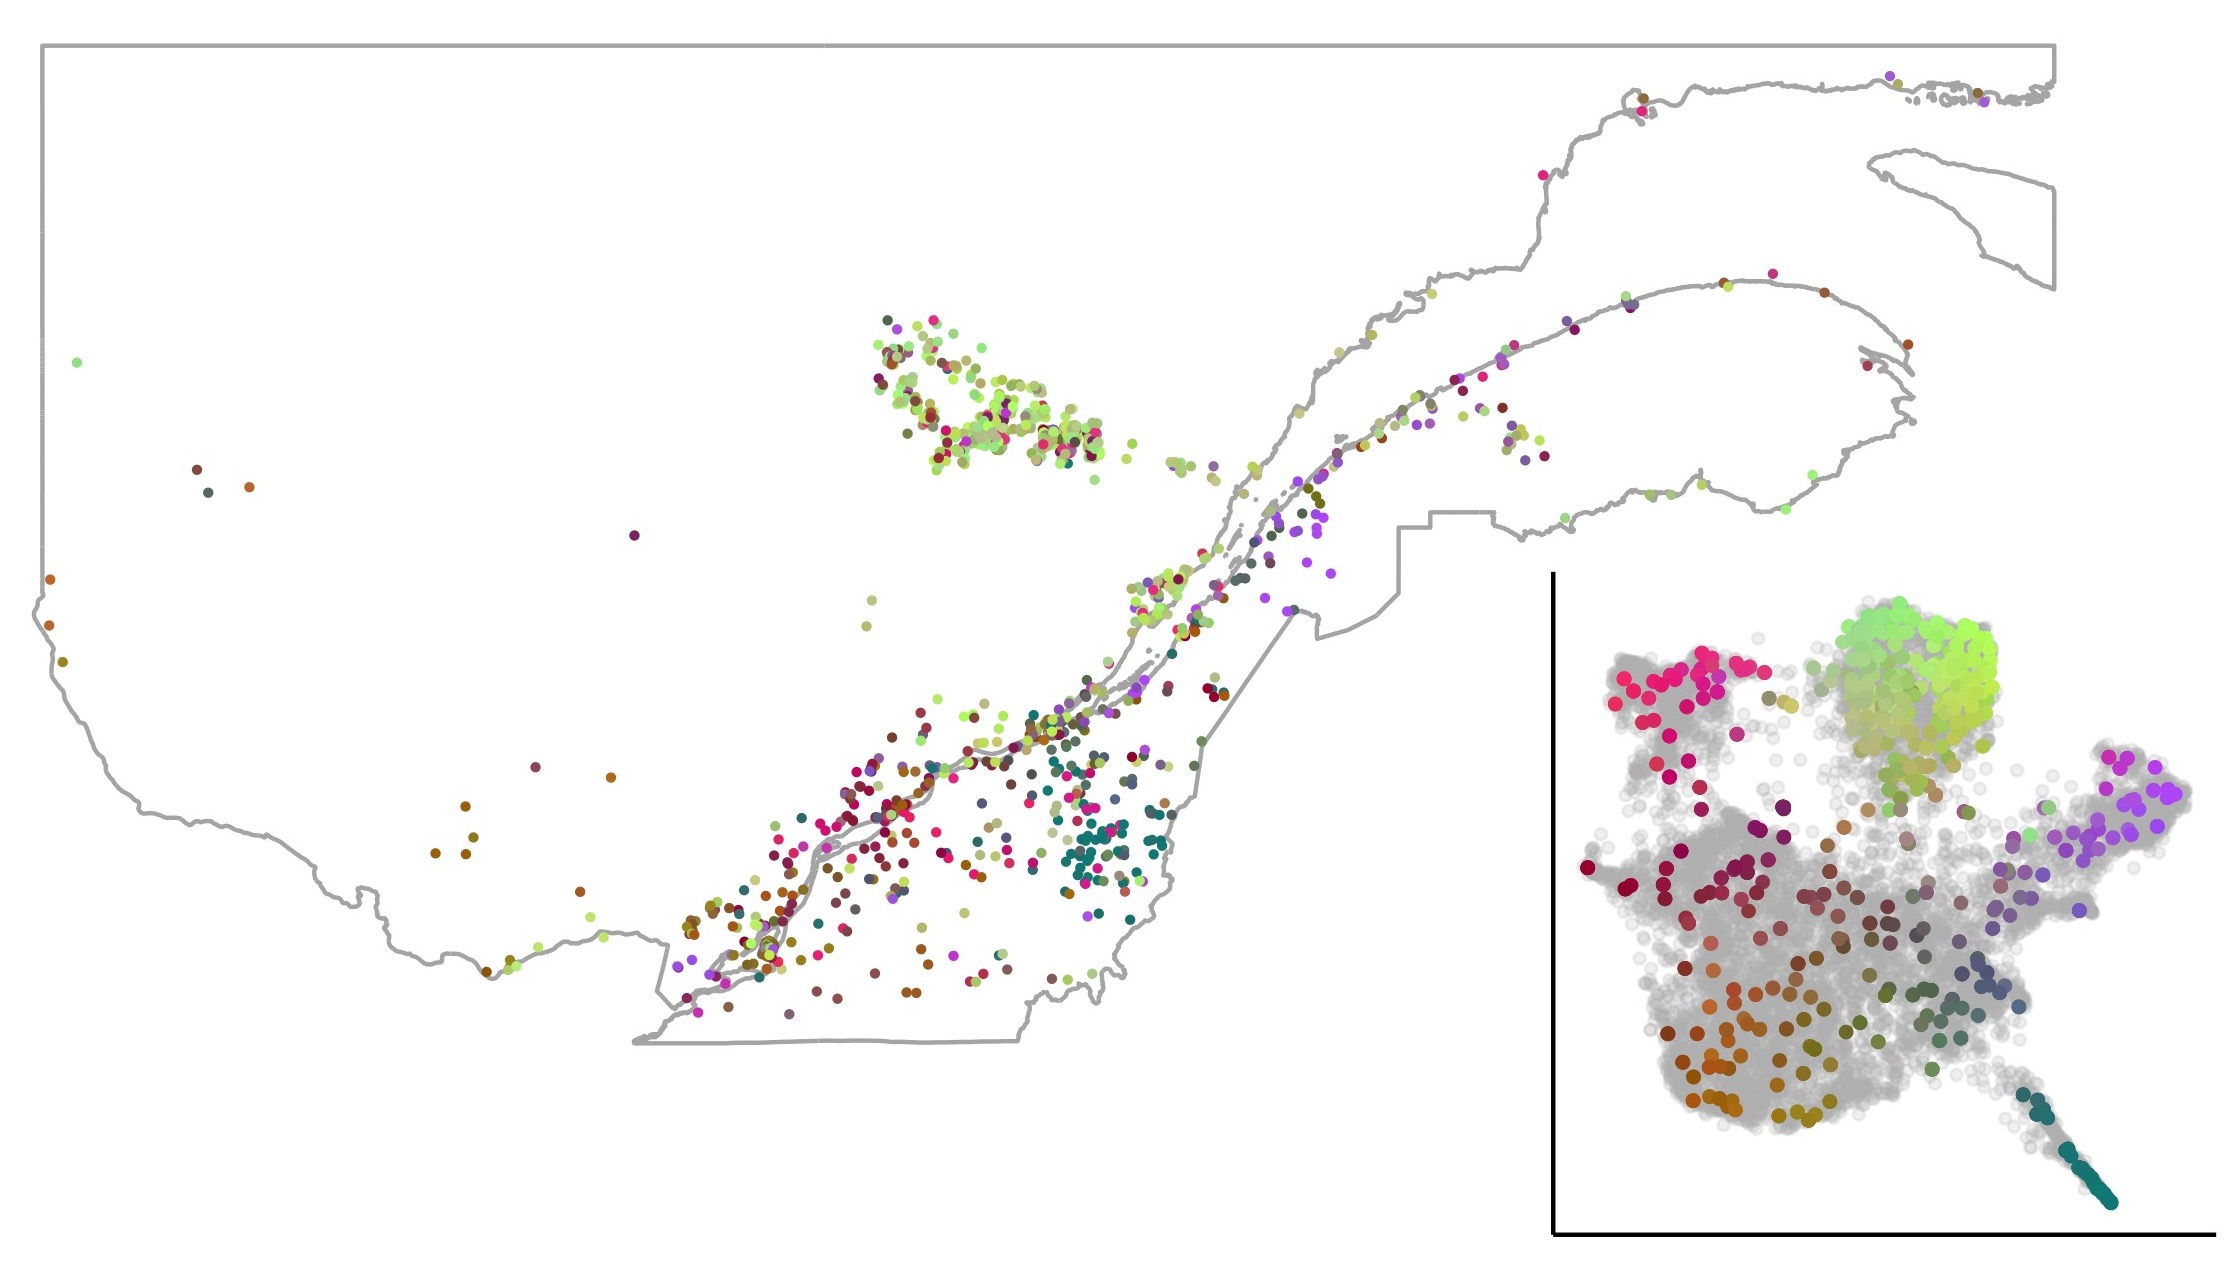
\includegraphics[width=\hsize,keepaspectratio]{./Figures/Genizon_BalSac_mapsInMaps4.jpg}
\label{UMAP}
\end{figure}


\section{Future Directions}
We know that there are regional differences in disease rates that are linked to population substructure.
The genetic data used in UMAP analysis also identify similar clusters.
Identifying the variants that are responsible for the clustering could also provide us with a shortlist of variants that could also be linked to the diseases that are associated with these sub-populations.
This method has yet to be formalized, but in brief, performing a logistic regression predicting presence of genotypes using the axis of variation that separates one group from the others could be used to identify these variants.

Expanding the current analyses to include data from French individuals could be used to confirm the results from the Fst analysis as well as provide insight into which regions in France are source populations to regions in Quebec. 

\chapter{Estimating mutation rates}

\section{Review of current methods and limitations}
Three main categories of methods :

1. Phylogenetic rate : Chimp vs human estimates 2.5 x 10-8 but limitations about the number of generations that separate the two species. Based on fossil evidence.

2. Direct approach : One generation using trio sequencing. 
Tend to give lower estimates compared to phylogenetic approach. (1-1.25 X10-8)

Pedigree approaches are simple in and direct approaches for per generation estimates but are met with several limitations.
Sex bias : fathers germline mutations increase with age and could be different among men.
Difficulty distinguishing difference between mosaicism and germline/somatic mutations.

Using Trio : sequencing tech limitations in error rates.
Mosaicism in parent or postzygotic mutations in child.
Father's age : spermatogenesis cell division.
Different types of mutations occur at different rates (and changes with age)

Converting per generation to per year is also difficult. 
Current approach is to divide generation rate by age of reproduction. (assumes same reproductive age for all pops over all time)
Estimates may only be accurate to the population studied. 

Mutational signatures specific to populations suggest recent changes in mutation rates. 

One possible solution is to limit estimates to CpG sites as they appear to have more consistent mutation rates across primates. *(but apparently no diff in paternal age for CpG transitions vs other mutations)

3. Population genetics approach : 
Estimates around 1.6-1.7 x 10-8

Taking advantage of founder populations with known pedigrees can get better estimates of mutation rates over multiuple generations.
Identify mutations in regions of autozygosity and count the number of generations that separate these segments. 
Reduces errors from somatic mutations. 
\subsection{Approach and methods for new calculation}

\subsection{Apply state of the art methods to new data}

\subsection{can we do better?}
Estimating mutation rate spatially across the genome.
Using IBD and Genealogy to better estimate the number of generations.

%----------------------------------------------------------------------------------------
%	THESIS CONTENT - APPENDICES
%----------------------------------------------------------------------------------------

\appendix % Cue to tell LaTeX that the following "chapters" are Appendices

\begin{figure}
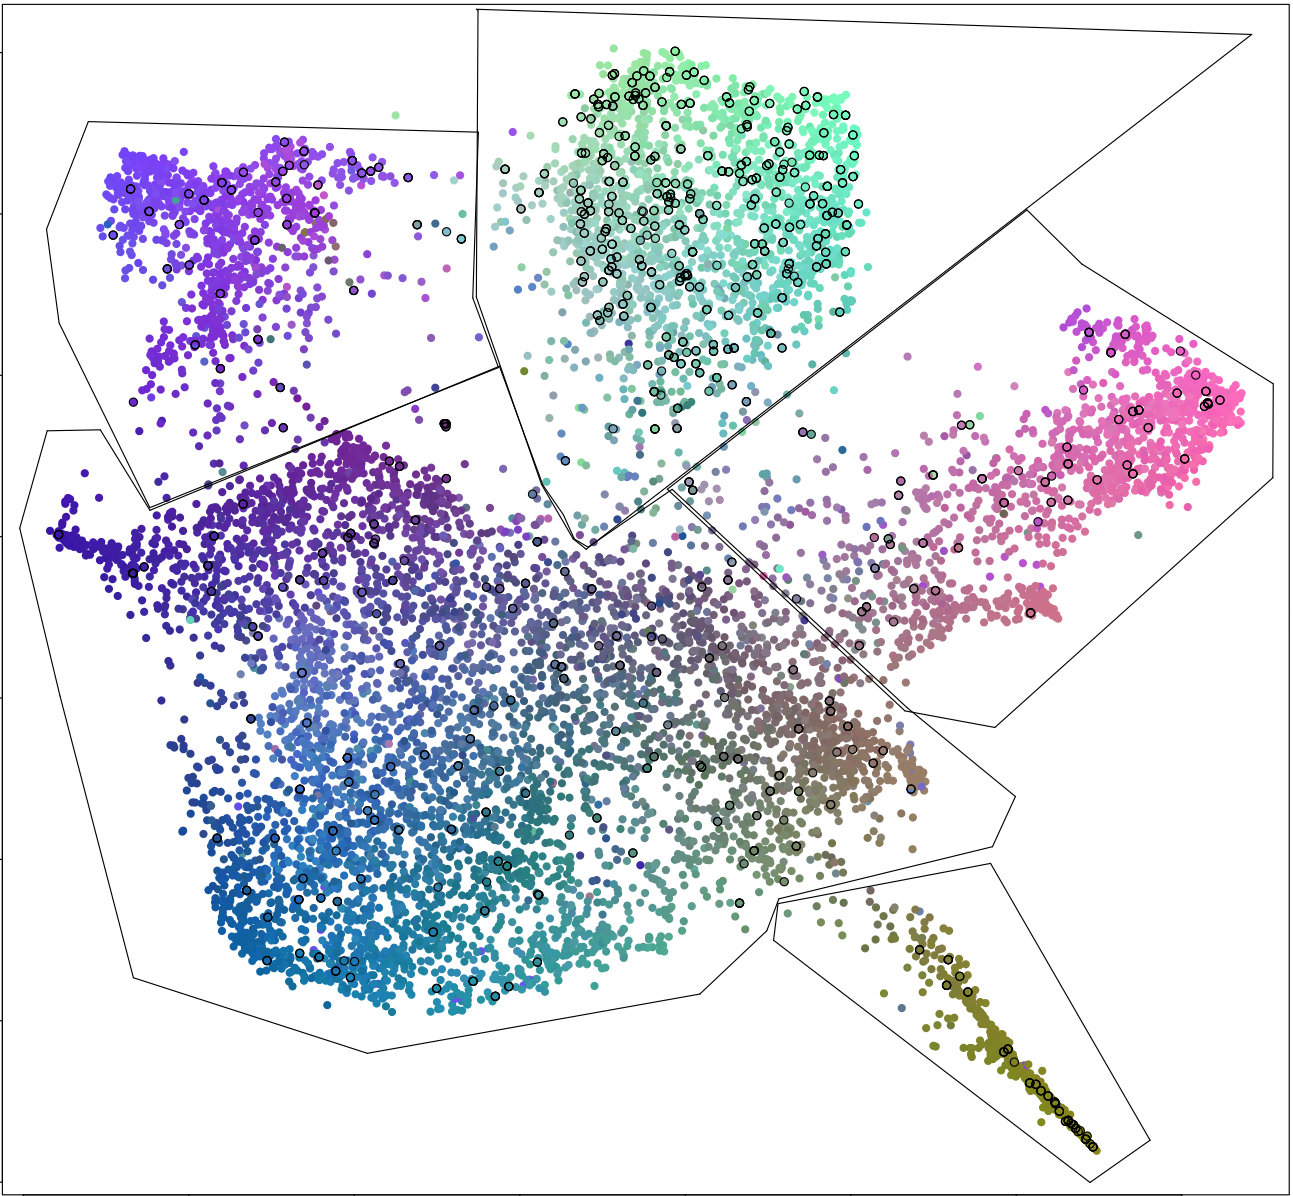
\includegraphics[width=\hsize,keepaspectratio]{./Figures/5Clusters.png}
\label{Cluster}
\end{figure}

% Include the appendices of the thesis as separate files from the Appendices folder
% Uncomment the lines as you write the Appendices

%\include{Appendices/AppendixA}


%----------------------------------------------------------------------------------------
%	BIBLIOGRAPHY
%----------------------------------------------------------------------------------------

\printbibliography[heading=bibintoc]

%----------------------------------------------------------------------------------------

\end{document}  
